\documentclass[11pt,preprint]{aastex}
 \begin{document}

\title{SUGGESTIONS FOR LAB REPORTS---\today}

\section{A Typical Outline for a Scientific Paper}

A typical scientific paper is divided into sections, subsections, and
subsubsections. The global outline for a typical scientific paper looks
like the following. Note, however, that there are wide variations from
this, which depend on content, subject matter, and individual
style. \begin{enumerate}

\item Title. Should encapsulate the contents and meaning.

\item Abstract. A short summary of the paper including the most important
  results.  Purpose is to tell a prospective reader whether it is worth
  spending more time on article.
  
\item Introduction. Sets the context: summary of the current state of
  knowledge, how that state can be improved, what this work does to
  advance the field. What did you hope to accomplish? Briefly, what did you
  accomplish? 

\item Observations or Experiments. What you observed, who did it, when you
  did it, what equipment you used, how you recorded data, any particulars
  or peculiarities.

\item Data Analysis. The theory according to which you analyze the data,
  how you actually did the analysis, the results of your analysis. Provide
  the essential numbers---the distillation of your original data (often
  millions of numbers) into a set of essential numbers or results. This is
  what we mean by ``data reduction''!

\item Interpretation. What the results mean in terms of astrophysics or
  your previous state of knowledge. How your results relate to specific
  issues that were mentioned in the introduction.

\item Conclusion. A summary of important results and points made in the
  paper, including pointing to the particlar sections so that the reader
  can easily learn more detail. What aspects are lacking? How would
  you have done things better? Prospects for future work.
  

\end{enumerate}

\section{Scientific and Interpretive Issues}

	These are {\it most important} because they related directly to
your scientific and experimental work and interpretation. 
\begin{itemize}

\item When you derive a result or calculate something it's important to
be {\it self-critical}. This is known as a {\it reality check}. Various forms
of reality check include the following (a limited list):
\begin{enumerate}

	\item Generate fake data. Run your software on them ({\it note
the plural use of ``data''!}) and check for consistency. 

	\item When doing a least-squares fit, plot the {\it data},
overplot the {\it fitted curve}, and plot the {\it residuals}. The data
and fitted curve should look similar. The residuals should exhibit no
systematic trends and should look like noise clustered around zero. If
not, why not?

	\item Before deriving a result with fancy numerical techniques
you should first make a guess, using your physical intuition, about what the
answer is. If your fancy numerical technique gives something wildly
different, then  \begin{enumerate}

	\item Your physical intuition is no good, which means you don't
understand the basic fundamentals. 

	\item Your numerical technique or software is no good.
\end{enumerate}

\noindent Which is it? (Or is it both????) Talk to people, ask
questions, or whatever, but {\it resolve these discrepancies!}

\end{enumerate}

	\item When you plot some data, {\it look at the plot and
think about what you see}.  For example, when you observed the Sun
with the interferometer, the Campanile shadowed the dishes and the
signal went away for some time.  Ask yourself: what happened to the data
during that time? In your lab report, such things are worth comments!

\item Abstracts should contain essential information---{\it including the
important numbers that you derive}. 

\end{itemize}

\section{ Grammar, etc.}

	Some grammatical-type issues: \begin{itemize}

	\item The word `data' is {\it plural}. Use it as you would use
the word `datapoints'. The singular of data is {\it datum}. Use it as
you would use the word `datapoint'. For example: \begin{enumerate}

	\item The data {\it indicate} (not {\it indicates!}) that the
system doesn't work\dots Similar to saying ``The datapoints
indicate\dots''

	\item This datum {\it is} a bad measurement and we will discard
it.  
\end{enumerate}

	\item Capitalize proper names. This includes `Fourier', `Gauss'
or `Gaussian', `Sun', `Moon', `Orion', etc.

	\item Check spelling! From the UNIX prompt, type

\begin{verbatim}
ispell -t mylab.tex
\end{verbatim}

\noindent which runs an interactive spell checker. The \verb$-t$ means
``ignore TEX-related commands''. Spell checking isn't a panacea because a
typo can produce a properly spelled word that isn't appropriate.
Example: ``These data are like ship.''

\end{itemize}

\section{ Plotting/IDL Issues} \label{plotting}

	Some plotting- or IDL- related issues: \begin{itemize}

	\item Axis labels and annotations on plots need to be large
enough to be legible.  Also, you really ought to use nice fonts: don't
underestimate the value of good looks! And you usually want thicker
lines. To accomplish all this in postscript the cumbersome way is to
specify a lot of stuff in {\tt psopen}; the easy way is to use our canned
wrapper procedure {\tt ps\_ch}:

\begin{verbatim}
ps_ch, 'outputfile.ps', /defaults, xsize=5, ysize=6, /inch
plot, x, y, xtitle='This is X', ytitle='This is Y', title="Carl's plot"
ps_ch, /close
\end{verbatim}

\noindent You can look inside this procedure to see how to change font
size and line thicknesses. See Figure \ref{simple}.

\begin{figure}[b!]
\begin{center} \leavevmode
%\includegraphics[scale=.7]{simple.ps}
%\includegraphics[scale=.8]{nicer.ps}
\includegraphics[scale=.55]{simple.ps}
\includegraphics[scale=.6]{nicer.ps}
\end{center}
\caption{Left: Titles are too small, lines too thin, font doesn't look
good. Right: Nicer! (But it could be even nicer!!) See \S
\ref{plotting}.  \label{simple}}
\end{figure}
                                                                        

	\item When plotting datapoints, it's usually a good idea to plot
the points themselves, which you'd do with the keyword \verb$psym=4$,
for example \footnote{Or some other number---the number gives the plot
symbol shape.}.  Sometimes you also want to connect the datapoints with
lines, which you do with \verb$psym=-4$.  Or---especially when you do
least squares fits---you want to overplot the datapoints with a fitted
curve; to do this, plot the datapoints and then use \verb$oplot$ to
overplot the curve. 

\item If you want to evaluate fancy mathematical functions you don't
need to use Mathematica.  IDL has all those functions too.  For example,
from the IDL prompt, type \verb$?gamma$ to get info on the Gamma
function.  A software language is just that---a {\it language}---and the
more proficiently you speak it, the better off you are.  It's a really
bad idea to use different software for different jobs when you don't
have to. 

\end{itemize}

\section{TEX hints}

	Some TEX hints: \begin{enumerate}

	\item Mathematical convention says: usually, write
$(R^2-x^2)^{1/2}$ instead of $\sqrt{R^2-x^2}$.  In TEX, the scripts are
\verb$(R^2-x^2)^{1/2}$ and \verb$\sqrt{R^2-x^2}$. 

	\item When you're doing complicated parenthetical expressions,
it's nice to use embedded sizing. TEX does this automatically for you:
instead of the not-very-elegant

$$ x = \cos [2\pi({B_y \over \lambda} cos(\delta))sin(h)] $$

\noindent you can write

$$ x = \cos \left[ 2\pi \left( {B_y \over \lambda} cos(\delta) \right) sin(h) \right] $$

\noindent The scripts for these are

\begin{verbatim} 
$$ x = \cos [2\pi({B_y \over \lambda} cos(\delta))sin(h)] $$

and

$$ x = \cos \left[ 2\pi \left( {B_y \over \lambda} cos(\delta) \right) sin(h) \right] $$
\end{verbatim}

\noindent Note the (double) use of \verb$\left[$ and \verb$\right$] . 
Also, note the Roman letters for the trig function, i.e.\ convention
prefers $\cos(ha)$ instead of $cos(ha)$; we accomplish this in TEX by
writing \verb$\cos(ha)$ (note backwards slash in \verb$\cos$) instead of
\verb$cos(ha)$. 

\item You can print a Table of Contents by writing
\verb$\tableofcontents$ in your TEX document (usually at the beginning,
but you can do it anywhere). This is very helpful when
organizing your lab report into sections and subsections.

\item You can get the proper looking quotes, either `single' or
``double'', by writing \verb$`single'$ or \verb$``double''$ . 

\item You can get a proper ``times'' sign, as in $2 \times 3$, using
\verb=$2 \times 3$=. 

\item You can get equations numbered 1a, 2b, and 3c instead of 4, 5,
and 6 by using the \verb$mathletters$ environment like this:
\begin{mathletters}
\begin{equation}
x = \sin (y)
\end{equation}
\noindent and then you can insert as much text as you want and\dots
\begin{equation}
z = \tan (y)
\end{equation}
\begin{equation}
u =  y^{1/2}
\end{equation}
\end{mathletters}
by typing the following:
\begin{verbatim}
\begin{mathletters}
\begin{equation}
x = \sin (y)
\end{equation}

\noindent and then you can insert as much text as you want and\dots

\begin{equation}
z = \tan (y)
\end{equation}
\begin{equation}
u =  y^{1/2}
\end{equation}
\end{mathletters}
\end{verbatim}

\item And finally, you can insert things verbatim into TEX, without the
TEX translations, by using \verb=\verb$verbatim into TEX$= (all must be
on one line) or, for multiple lines, get into the \verb$verbatim$
environment by typing

\begin{verbatim}
\begin{verbatim}
Now we are in the verbatim environment
Here is a multiple line situation
\end{verbatim}
\verb$\end{verbatim}$

\end{enumerate}
\end{document}

if ps then psopen, 'outputifile.ps', /times, /bold, /isolatin1
plot, x, y, xtitle='This is X', ytitle='This is Y', title="Carl's plot", $
        font=ps-1, charsize=1.5, thick=3, xthick=5, ythick=5
if ps then psclose
